

\subsection{Planification}

\paragraph{Partage des tâches}
Au départ de ce projet nous avions trois premiers objectifs, créer un outil de génération de carte en c++, poser les base du moteur de jeu en typescript et préciser le design du jeu que nous voulions créer. Nous nous sommes donc partagés les tâches, Tom Zink s’occuperait du moteur, Clément Saperes du game design, Kai Night et Timothée Bonetti de la génération de la carte.
Une fois les bases du moteur de jeu crées nous devions mettre en commun et créer les 2 gameplay, les interfaces, l'interactivité.
Cela a été plus compliqué que prévu, au vu de notre emplois du temps mais aussi de difficultés rencontrés: Mauvaise connaissances des technologies (typescript, TREE js), l'absence de librairie satisfaisante pour créer des interface utilisateur sur navigateur et autres soucis.

Nous explorerons plus en détails les difficultés rencontrés dans d'autres sections de ce compte rendu.

\begin{figure}[!h]
    \centering
    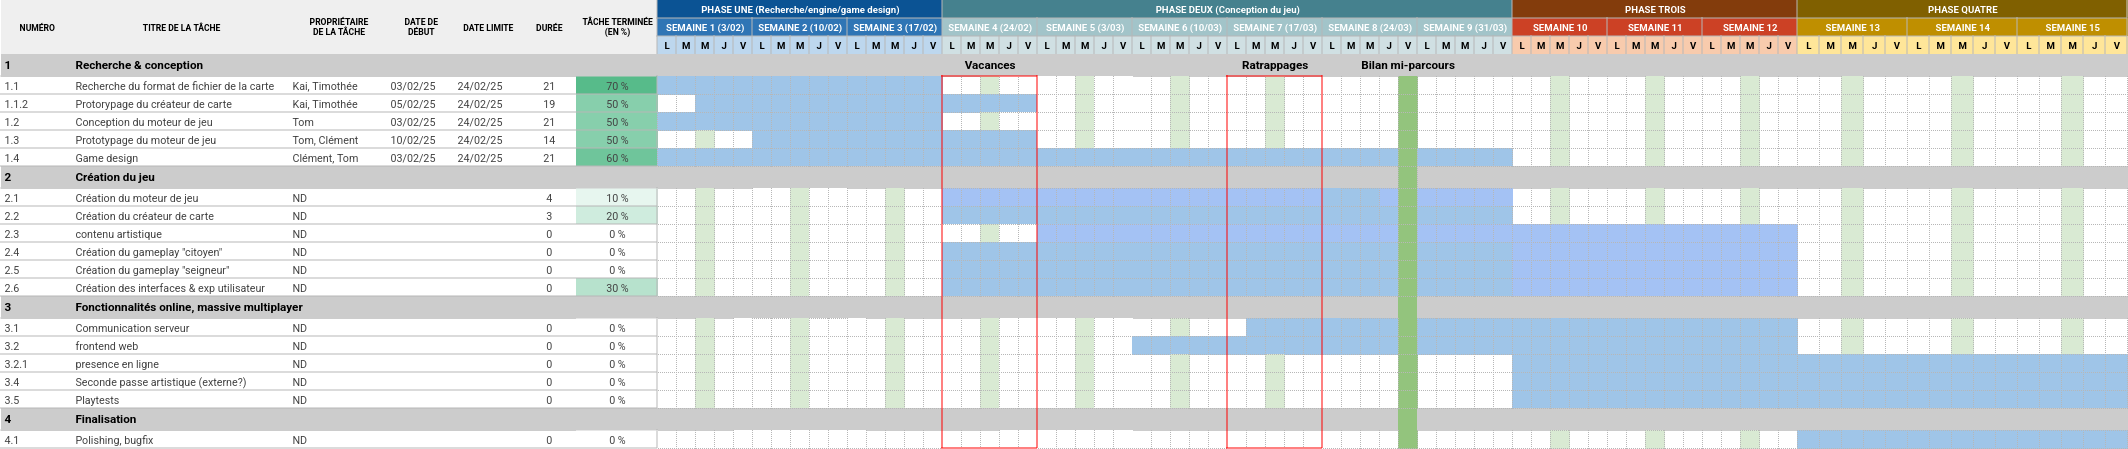
\includegraphics[width=0.99\linewidth]{images/gantt.png}
    \caption{Diagramme de Gantt}
    \label{fig:enter-label}
\end{figure}

Ce diagramme montre notre organisation initiale pour ce projet.